\chapterimage{uvdisinfectionhero.jpg} % Chapter heading image

\chapter{Disinfection}

\section{Background}\index{Background}
\begin{itemize}
\item The primary goal of water treatment is to ensure that the water is safe to drink and does not contain any disease-causing microorganisms. 
\item Disinfection refers to an operation to inactivate the microorganisms in water that can cause an infection or disease. These organisms are collectively referred to as pathogens and include many species of bacteria, fungus, protozoa, worms, viruses, etc.
\item The processes prior to disinfection - sedimentation and filtration, remove a large percentage of bacteria and other microorganisms from the water by physical means.
\item Disinfection is different from sterilization, which is the complete destruction of all organisms which is expensive and unnecessary.
\item Water disinfection can be sub-divided as:
\begin{enumerate}
\item Primary disinfection:
\begin{itemize}
\item Kills or inactivates bacteria, viruses, and other potentially harmful organisms in drinking water.
\item Disinfection prevents infectious diseases such as typhoid fever, hepatitis, and
cholera
\item Some disinfectants are more effective than others at inactivating certain
potentially harmful organisms.
\item Disinfection processes vary from water utility to water utility based on their
needs and to meet EPA treatment requirements.
\end{itemize}
\item Secondary disinfection:
\begin{itemize}
\item Maintenance of a disinfectant residual that prevents regrowth of microorganisms in the water distribution system between treatment and consumer.
\item Secondary disinfection maintains water quality by killing potentially harmful
organisms such as those that cause Legionnaire’s disease that may get in water as it moves through pipes.
\item Monochloramine is commonly used as a secondary disinfectant.
\end{itemize}
\end{enumerate}
\item Elements of an "ideal" disinfectant
\begin{itemize}
\item It must act in a reasonable time.
\item It must act as temperature or pH changes.
\item It must be nontoxic.
\item No harmful byproducts.
\item It must not add unpleasant taste or odor.
\item It must be readily available.
\item It must be safe and easy to handle and apply.
\item It must be easy to determine the concentration of.
\item It must be able to provide residual protection.
\item Pathogenic organisms must be more sensitive to the disinfectant than are nonpathogens.
\item It must be capable of being applied continually.
\item Versatile:  effective against all types of pathogens.
\item Fast-acting:  effective within short contact times
\item Robust: effective in the presence of interfering materials including particulates, suspended solids and other organic and inorganic constituents
\item Handy: easy to handle, generate, and apply (nontoxic, soluble, non-flammable, non-explosive)
\item Compatible with various materials/surfaces in WTPs (pipes, equipments)
\item Economical
\end{itemize}
\item In addition to the desirable characteristics of a disinfectant listed above, the disinfectant chosen must be able to kill off or deactivate pathogenic microorganisms by one of several possible methods, including:
\begin{enumerate}
\item Damaging the cell wall
\item Altering the ability to pass food and waste through the cell membrane
\item Altering the cell protoplasm
\item Inhibiting the cells’ conversion of food to energy
\item Inhibiting reproduction
\end{enumerate}
\end{itemize}

\section{Chlorination}
\begin{itemize}
\item Despite potential drawbacks, chlorine is the disinfectant of choice.
\item In general, chlorination is effective, relatively inexpensive, and provides effective levels of disinfectant residual for safe distribution. 
\item Chlorine can be applied as:
\begin{itemize}
\item As a gas - elemental chlorine, $\mathrm{Cl}_{2}$:\\
\item Liquid (sodium hypochlorite) 
\item Solid (calcium hypochlorite)\\
each of these forms has advantages and disadvantages.
\end{itemize}
\end{itemize}
\subsection{Chlorine properties}\index{Chlorine properties}
\begin{itemize}
\item Chlorine is a yellowish-green gas at room temperature and atmosphric pressure
\item Chlorine gas can be pressurized and cooled to its liquid form for making it easy to ship and store. 
\item When liquid chlorine is released, it quickly turns into a gas that stays close to the ground (being heavier than air) and spreads rapidly.
\item While it is not explosive or flammable, as a liquid or gas it can react violently with many substances 
\item Chlorine is only slightly soluble in water (0.3 to 0.7\% by weight.) 
\item Chlorine gas has a greenish-yellow color 
\item It has a characteristic disagreeable and pungent odor, similar to chlorine-based laundry bleaches, and is detectable by smell at concentrations as low as 0.2 to 0.4 ppm
\item It is about two and a half times as heavy as air
\item One volume of liquid chlorine yields about 460 volumes of chlorine gas. 
\item Liquid chlorine is amber in color and is about one and a half times as heavy as water 
\item Chlorine is an irritant to the eyes, skin, mucous membranes, and the respiratory system 
\end{itemize}

\subsection{Chlorine storage and safety}\index{Chlorine storage and safety}
\begin{itemize}
	\item Chlorine gas is lethal at concentrations as low as $0.1 \%$ air by volume. In nonlethal concentrations, it irritates the eyes, nasal membranes, and respiratory tract.
	\item Typically for smaller plants chlorine gas is shipped in  pressurized steel cylinders - 150 lb or 2000 lb (ton cylinder) size.  Larger plants may get their chlorine supply in rail tank cars.  
	\item The daily chlorine usage is typically established based upon the weighing of the chlorine containers.
	\item The withdrawal rates from a chlorine cylinder is based on the temperature of the liquid in the cylinder, and thus the pressure of the gas. 
	\item As chlorine gas is withdrawn from the cylinder, it absorbs the heat from the surroundings.
	\item For low withdrawal rates, heat will be able to be transferred from the surrounding air to the container in time so that there is no drop in temperature or pressure, 
	\item If the chlorine withdrawal is larger, the air will not be able to transfer the heat quickly enough and the temperature (and pressure) of the chlorine will drop, thus resulting in a lower feed rate. 
	\item If high enough and prolonged enough, this can even result in ice formation around the outside of the container, further decreasing the withdrawal rate. 
	\item The most effective way to increase withdrawal rate from a single container is to circulate the surrounding air with a fan. Again, never apply heat to the containers.
	\item If chlorine gas escapes from a container or system, being heavier than air, it will seek the lowest level in the building or area
	\item Only trained staff with access to proper personal protection equipment (PPE) including self-contained breathing apparatus, should handle the chlorine cylinders and address chlorine leak issues 
	\item When a leak is suspected, it is recommended that ammonia vapors be used to find the source. When ammonia vapor using a rag or brush, is directed at a leak, a white cloud will form. To produce ammonia vapor, a plastic squeeze bottle containing about 5 \% ammonia, aqua ammonia (ammonium hydroxide solution) should be used. A weaker solution such as household ammonia may not be concentrated enough to detect minor leaks
	\item All safety equipment should be located outside of the chlorine room and be easily accessed by all personnel
	\item Small leaks around valve stems can usually be corrected by tightening the packing nut or closing the valve. A leak can also be reduced by removing the chlorine as rapidly as possible
	\item If it cannot be added to the process there are several chemicals which can be used to absorb the chlorine gas. For example, chlorine can be absorbed by using 1$frac{1}{4}$ pounds of caustic soda or hydrated line, or 3 pounds of soda ash per pound of chlorine. 
	\item If the leaking container can be moved, it should be transported to an outdoors area where minimal harm will occur. Keep the leaking part the most elevated so that gaseous chlorine will leak rather than liquid chlorine.
	\item If the leak is large, all persons in the adjacent area must be warned and evacuated. Only authorized persons equipped with the proper breathing apparatus, and protective measures to the eyes and body should investigate. 
	\item As water is not an efficient absorbent for chlorine and the fact that chlorine reacts with water to form very corrosive hydrochloric acid, never apply water to a leak or consider submerging a chlorine cylinder (for example, in a pond or tank), since it will probably float.
	\item Remember to keep windward of the leak.
	\item As chlorine cylinders pressure increases with temperature, as a safety measure the chlorine cylinders are fitted with fusible plug which melts between 158$^o$ and 165$^o$ F.
	\item Keep chlorine cylinder or container emergency repair kits available. Be familiar with their use and location.
	\item Leaks at fusible plugs and cylinder valves requires special handling and emergency equipment. The chlorine supplier must be notified immediately
	\item Pin hole leaks in cylinder walls or ton tanks can usually be stopped by mechanical pressure applications (clamps, turnbuckles, etc.). This only temporary and may require your ingenuity.
	\item Leaking containers cannot be shipped.
	\item In general, daily inspection of all chlorine cylinders will avoid major problems\\
	
\end{itemize}

\subsection{Forms of chlorine}\index{Forms of chlorine}

\begin{itemize}
	\item Due to safety issues related to the use of chlorine gas, \textbf{hypochlorites} are often used in lieu of chlorine
	\item Types of hypochlorites
	\begin{itemize}
	\item Sodium hypochlorite (NaOCl) comes in a liquid form which contains up to 12.5\% chlorine
	\item Calcium hypochlorite (Ca(OCl)$_2$), also known as High-test Hypochlorite (HTH), is a solid which is mixed with water to form a hypochlorite solution. Calcium hypochlorite is 65-70\% concentrated.
	\end{itemize}
	\item Hypochlorites decompose in strength over time while in storage. Temperature, light, and physical energy can all break down hypochlorites before they are able to react with pathogens in water. 

\end{itemize} 

\subsection{Chlorine reactions related to disinfection}\index{Chlorine reactions related to disinfection}


\textbf{Chlorine reacts with water to form hypochlorous and hydrochloric acids}\\
Cl$_2$ \hspace{0.8cm}	+ \hspace{0.3 cm}	 H$_2$O		\hspace{0.8cm} $\iff$ 
\hspace{0.8cm} HOCl	\hspace{0.8cm}	 +	\hspace{0.8cm}	 HCl \\
chlorine \hspace{0.8cm}	water \hspace{1.8cm}		 hypochlorous acid	\hspace{0.1cm}	 hydrochloric acid\\ 
	\vspace{0.5cm}
	\begin{itemize}
		\item Hypochlorous acid dissociates in water to form the hydrogen and hypochlorite ions\\
 HOCl \hspace{1.8 cm} $\iff$ \hspace{1.8 cm} H$^+$ \hspace{1.8cm} + 	\hspace{0.8cm}OCl$^-$\\ 
hypochlorous acid  \hspace{1.9 cm}      hydrogen ion   \hspace{1.5cm}           hypochlorite ion

		\begin{itemize}
			\item Hypochlorous acid is the most effective form of chlorine available to kill microorganisms
			\item Hypochlorite ions is much less efficient disinfectant
		\end{itemize}

		\item The concentration of hypochlorous acid and hypochlorite ions in chlorinated water will depend on the water's pH
		\begin{itemize}
			\item A higher pH facilitates the formation of more hypochlorite ions and results in less hypochlorous acid in the water
		\end{itemize}
		\item A significant percentage of the chlorine is still in the form of hypochlorous acid even between pH 8 and pH 9
		\end{itemize}


\subsection{Chlorine disinfection process}\index{Chlorine disinfection process}

\linespread{1.5}
\begin{itemize}
\item When chlorine is added to a wastewater flow, it will first react or combine with certain organic and inorganic substances present, prior to acting on pathogens.  The amount of chlorine used up as part of these reactions is referred to as the \textbf{chlorine demand}\\

\item The \textbf{free chlorine} remaining after the chlorine demand is satisfied, is the strongest form of chlorine available for disinfection.  

\item Chlorine combined with ammonia (as chloramines) and organic compounds (as chloroorganic compounds), known as \textbf{combined chlorine} also exhibit disinfecting properties - albeit weaker than the free chlorine.

\item \text{Total residual chlorine} is the sum of free chlorine and combined chlorine and it is the residual chlorine concentration which represents the amount of chlorine available for disinfection 
\end{itemize}
\textbf{Chlorine Demand = Applied Chlorine Dose - Chlorine Residual}\\

\subsection{Factors affecting chlorine disinfection}\index{Factors affecting chlorine disinfection}
The disinfection efficiency of chlorine depends on the following factors:\\
\begin{itemize}
	\item pH:  Disinfection is more efficient at a low pH when large quantities of hypochlorous acid are present than at a high pH when hypochlorite ions is the dominant species in the water
	\item Concentration:  Contact Time Ratio (CT):  For effective chlorine disinfection both sufficient chlorine dosages – concentration (C) as well as contact time (T) are necessary.   Generally both of these factors must be worked out experimentally for a given system
	\item Disinfection activity can be expressed as the product of disinfection concentration (C) and contact time (T) - CT
	\item The same CT values will achieve the same amount of inactivation
	\item Temperature:  Colder temperatures are less favorable for disinfection. 
Proper contacting or mixing or agitation:  This is necessary to make sure that the chlorine applied contacts or reaches the microbial cells
	\item Organic and inorganic material present:  The chlorine used by these organic and inorganic reducing substances including metal ions, organic matter and ammonia, is defined as the chlorine demand.  So that the amount of chlorine that has to be added to wastewater for different purposes will also vary.
\end{itemize}

\subsection{Chlorine Application}\index{Chlorine Application}
\begin{itemize}
\item Continuous chlorination of systems less than 75 gpm is by the use of a hypochlorinator where a motor driven pump pulls the hypochlorite solution out of a holding chamber and pumps it into the water to be treated.  Where the pipe from the pump joins the pipe carrying the raw water, the Venturi effect creates a small vacuum and pulls the chlorine solution into the water.
\item For larger system, chlorinators - devices which introduce chlorine gas to water using liquid chlorine supplied in steel cylinders are used.
\item In the commonly used Vacuum Chlorinator:
\begin{itemize}
\item Chlorine gas is pulled from the cylinder into the source water by a vacuum created by water flowing through the injector and creating a negative head. 
\item This negative head forces open the pressure regulating valve on the cylinder and allows chlorine gas to flow out of the cylinder and into the chlorinator.
\item Once the gas has entered the chlorinator, the chlorine feed rate is measured using an indicator known as a rotameter
\item Just beyond the rotameter, the chlorine gas flows past a regulating device (a V-notch plug or a valve) which is used to adjust the chlorine feed rate.
\end{itemize}
\begin{figure}[h]
\begin{center}
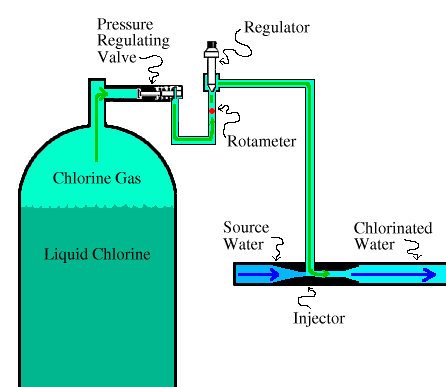
\includegraphics[scale=0.6]{VacuumChlorinator}\\
\captionof{figure}{Vacuum Chlorinator}%\caption{}
\end{center}
\end{figure}
\end{itemize}
\vspace{-2em}
\subsection{Chlorination Byproducts}\index{Chlorination Byproducts}
\begin{itemize}
\item Main drawback of chlorine disinfection is the adverse health effects of the byproducts - Disinfection by-products (\colorbox{pink}{DBPs}) formed from its reaction with certain organic compounds present in the water.
\item  Adverse health effects on humans exposed to DBPs through drinking-water and oral, dermal, and inhalational contact with chlorinated water, include cancers of vital organs.
\item Halogenated trihalomethanes (\colorbox{pink}{THMs}) and haloacetic acids (\colorbox{pink}{HAAs}) are two major classes of disinfection byproducts (DBPs) commonly found in waters disinfected with chlorine. 
\item At the present time, about 90\% of U.S. water utilities use chlorine to disinfect water. Although chlorine has virtually eliminated the risks of waterborne disease such as typhoid fever, cholera, and dysentery, recent studies have shown risks associated with byproducts of chlorine—a reason why water utilities already have been looking at alternative methods for disinfecting water.
\item Approaches for reducing DBPs includes:
\begin{itemize}
\item Avoiding pre-chlorination where chlorine is added to the raw water before coagulation and filtration.
\item Removal of organics using Aeration or adsorption on activated carbon 
\item reevaluating the chlorine dosing to a level which will accomplish the same degree of disinfection with a lower chlorine dosage.
\item Another current approach is using alternative disinfection methods.
\end{itemize}
\end{itemize}

\subsection{Chloroamination}\index{Chloroamination}
			\begin{itemize}
			\item When chlorine is added to water containing ammonia, chlorine reacts with ammonia to form chloramines.
						\item Chloramines has disinfection properties and although it is a weaker disinfectant than chlorine, it is more stable enabling to extend its disinfectant benefits through a wider range of the water distribution system.
						\item Additionally, water disinfection using chloramines provides benefit related to fewer taste and odor issues when compared to water disinfected with chlorine. 
					\item Water utilities practice chloroamination - practice of utilizing the disinfectant properties of chloramines, by feeding chlorine to the water containing ammonia.
			\item When chlorine is added to water containing ammonia, the :
			\begin{itemize}
				\item an initial absence of any increase in combined chlorine residual
				\item followed by a decrease in the combined chlorine residual
				along with ammonia concentrations
				\item followed by an increase in free chlorine residual and near complete removal 					of ammonia as nitrogen gas.\\
				\item Chlorine reacts with ammonia to form chloramines\\
				\begin{enumerate}
					\item First the free chlorine in contact with ammonia forms monochloramine and water
						\begin{itemize}
							\item Monochloramine has disinfection properties\\
							\item Dominates when Cl:N mass ratio is 0 to 5:1\\
							\item The breakpoint curve rises at about 1:1 during monochloramine formation\\
						\end{itemize}
					$NH_3 + HOCl   \rightarrow NH_2Cl (monochloramine) + H2O$\\
					\item Monochloramine reacts further with chlorine to give dichloramine and water\\
					$HOCl + NH_2Cl \rightarrow NHCl_2 + H_2O$\\
					Also, monochloramine auto decomposes into dichloramine\\
					$2NH_2Cl \rightarrow NHCl_2 + NH_3$
						\begin{itemize}
							\item Between dichloramine is formed between 5:1 and 7:1 Cl:N mass ratio
							\item When you are getting significant dichloramine, the breakpoint curve will start dropping
						\end{itemize}
						$NH_2Cl + HOCl  \rightarrow NHCl_2 (dichloramine)$\\
						at pH $>$ 7.5, monochloramine is the dominant chloramine species as pH decreases from 7.5, dichloramine becomes the dominant chloramine species increases in the chlorine to nitrogen dose ratio results in corresponding increases of nitrogen trichloride, but only when the pH is $<$ 7.4\\
					\item Formation of nitrogen trichloride from the reaction of chlorine and dichloramine does not typically occur as it is the favored product at low pH - $<$4\\
					$NHCl_2 + HOCl  \rightarrow NCl_3 (nitrogen trichloride)$\\
					\item Additional $free \enspace chlorine \enspace + chloramines \enspace \rightarrow H^+ + H2O + N_2$
				\end{enumerate}
				\item Chloramine levels up to 4 milligrams per liter (mg/L) or 4 parts per million (ppm) are considered safe in drinking water. At these levels, harmful health effects are unlikely to occur.				
				\item Chloramines have disinfection properties albeit much lower than free chlorine (~5\% of free available chlorine) but last much longer in the system than free chlorine. 
				\item Monochloramine is about 2,000 and 100,000 times less effective than free chlorine for the inactivation of E. Coli and rotaviruses, respectively.
				\item After the breakpoint, free chlorine residuals develop. Free chlorine residuals usually destroy odors, kill microorganisms and oxidize organic matter.
				\item Breakpoint chlorination is the application of sufficient chlorine beyond the chlorine demand to maintain a free available chlorine residual.\\  Theoretically chlorine requirement = Wt. NH$_3$-N x 7.6\\
				in practice (Margin of safety)     = Wt. NH$_3$-N x 10\\
				\item Thus, breakpoint chlorination is possible if ratio of Cl$_2$ to ammonia exceeds 10:1 then free Cl$_2$ may exist. Cl$_2$ demand will be high because the reaction of free Cl$_2$ with nitrite and other organic compounds. 
				\item Theoretically, while microorganisms are killed as the chlorine demand is being satisfied, disinfection is generally the result of chlorine residual or the amount of chlorine remaining after the chlorine demand has been satisfied.
			\end{itemize}
The following chart is a graphical explaination of the concept of Breakpoint Chlorination\\
			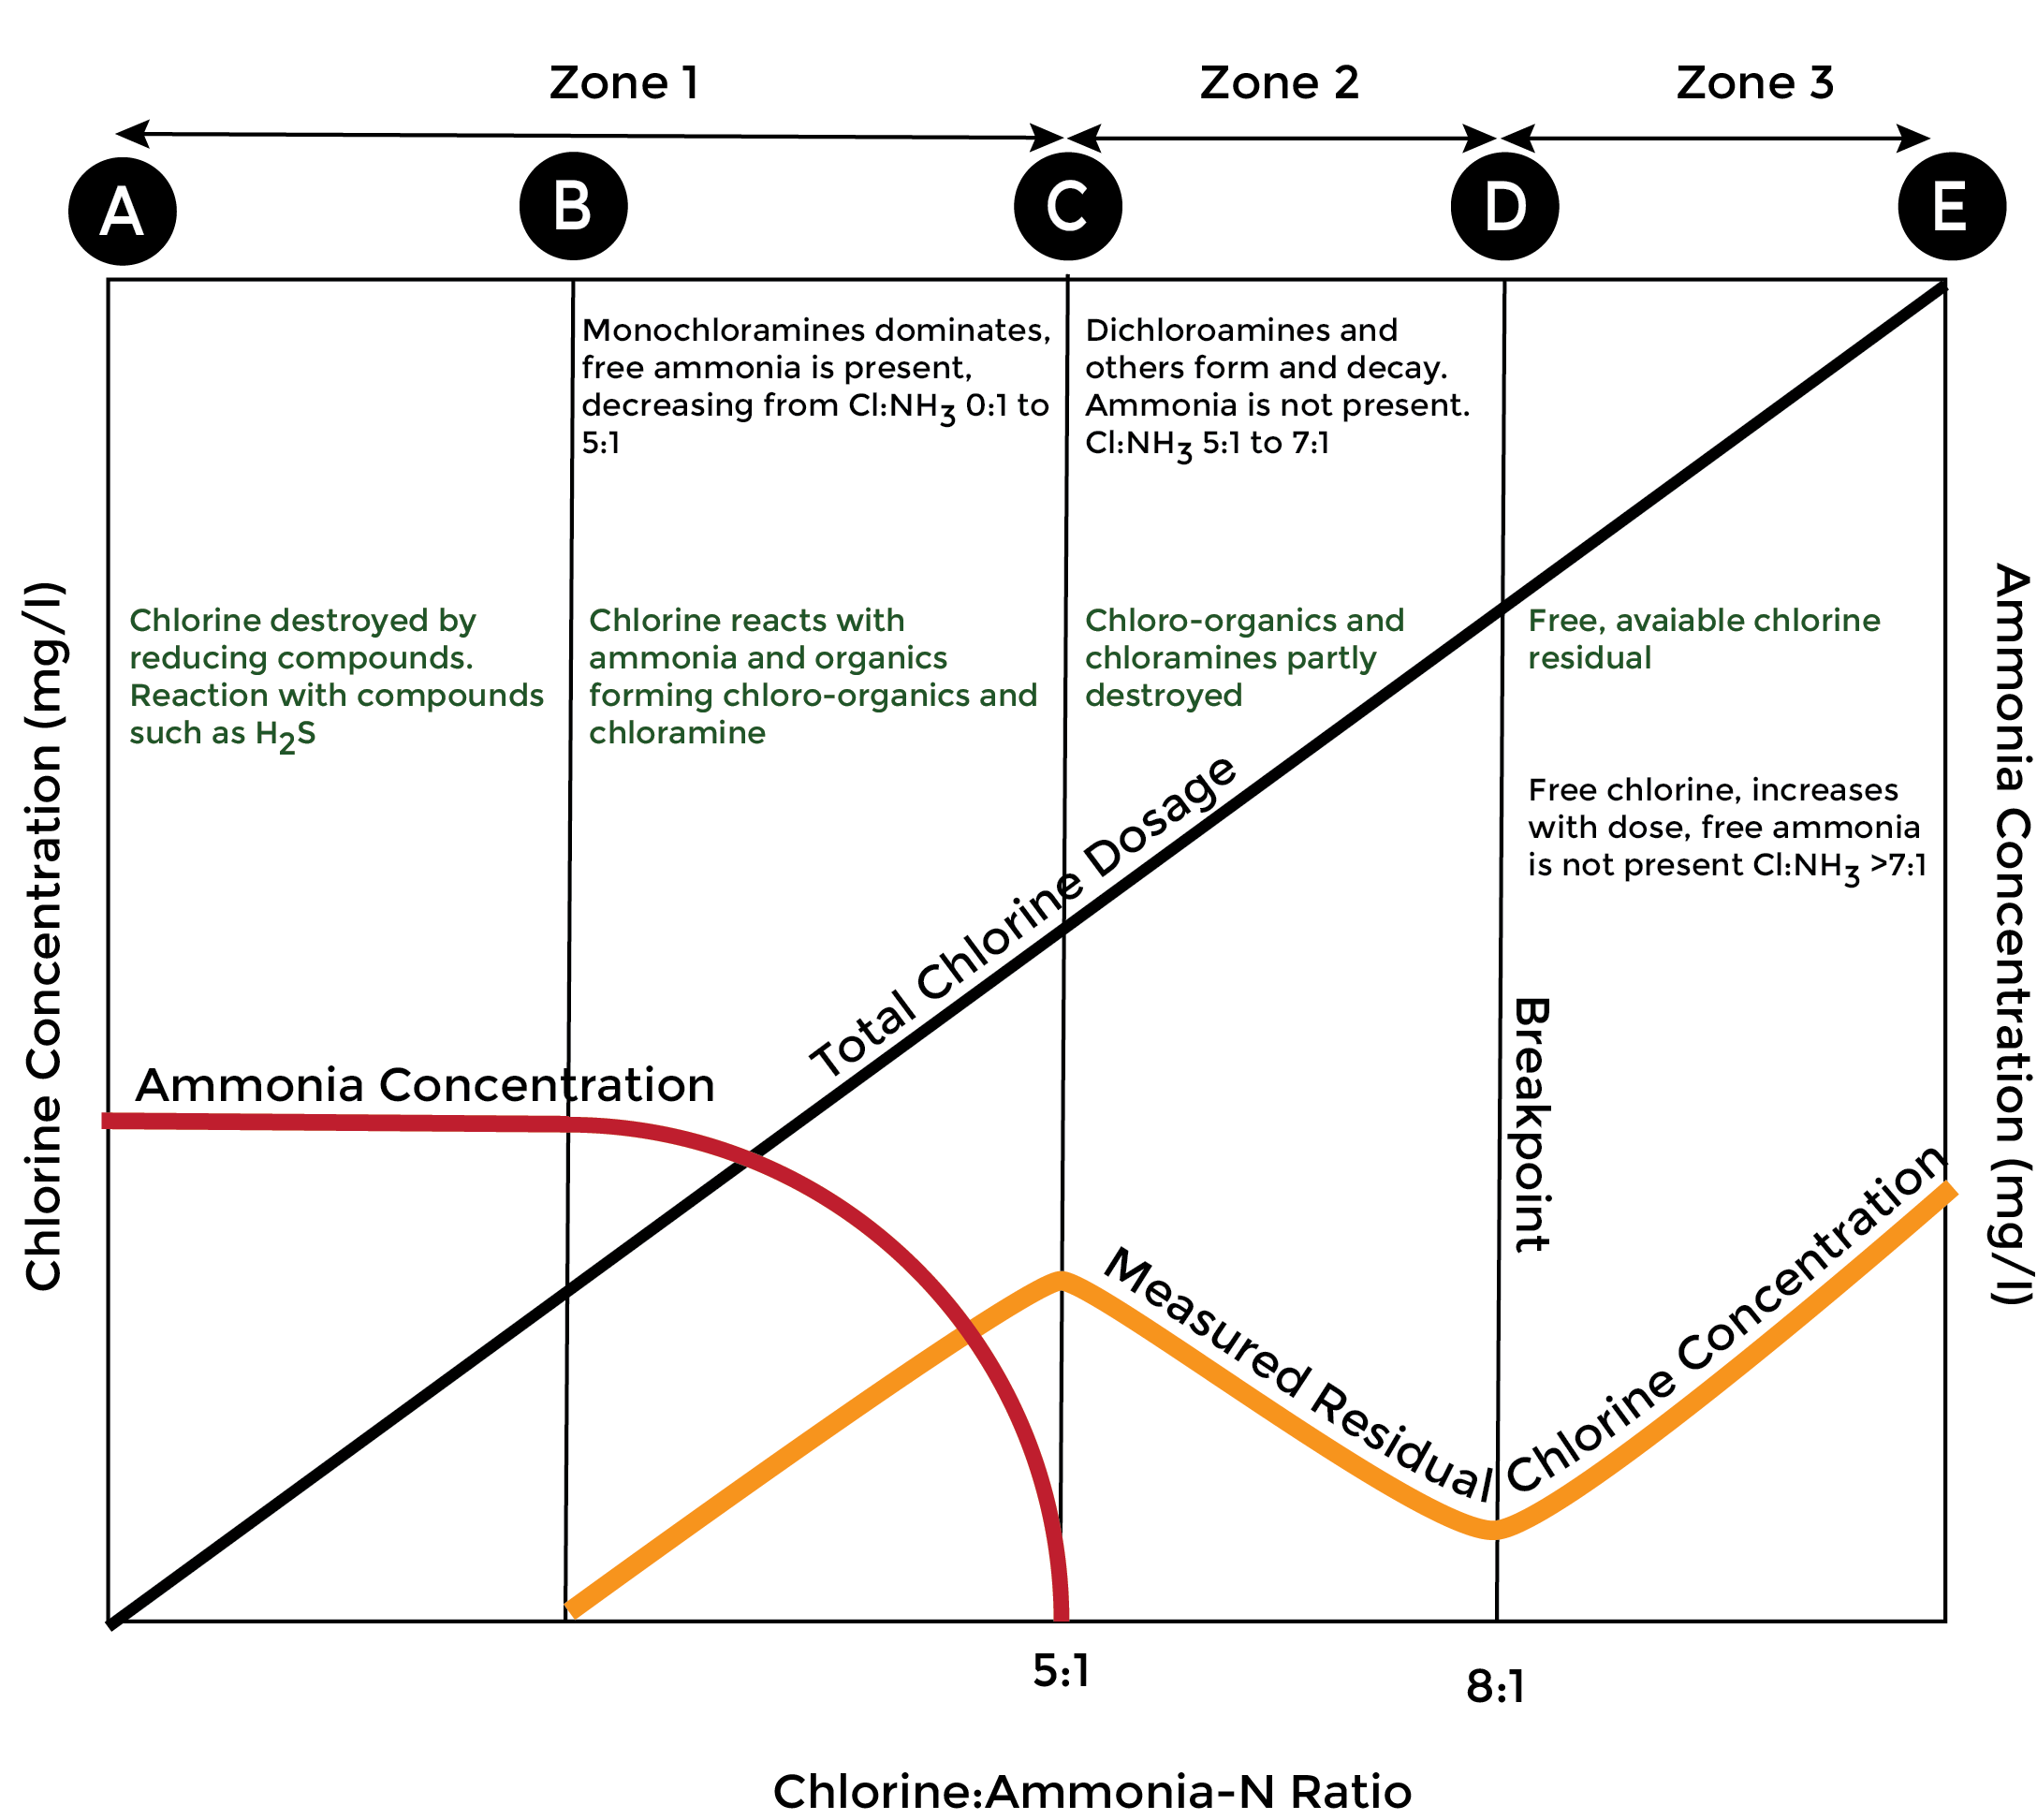
\includegraphics[scale=0.24]{BreakpointChlorination}
			\begin{itemize}
				\item Point A is at the beginning of chlorine application
				\item Between Points A and B, the chlorine dosage produces no residual because of an immediate chlorine demand caused by fast-reacting ions from metal salts and H$_2$S.
				\item Point B is the beginning of the reaction between chlorine and ammonia present
				\item Mono and dichloramines are formed between points B and C
				\item Zone 1 - between points A and C, is the combined zone and has mono and di  chloramines and ammonia.  Mono chloramines is a stable disinfectant while dichloramines is a strong disinfectant but unstable.
				\item After the maximum combined residual is reached (point C), further chlorine doses decrease the residual due to chloramine oxidation to dichloramine, occurring between points C and D.  This is Zone 2 - Breakpoint Zone
				\item Point D represents the breakpoint - the point at which chlorine demand has been satisfied and additional chlorine appears as free residuals
				\item Between points D and E, free available residual chlorine increases in direct proportion to the amount of chlorine applied.  This is Zone 3 which is the free chlorine zone and has hypochlorous acid but no ammonia. \\
			\end{itemize}
			\begin{itemize}
				\item Factors that affect breakpoint chlorination are initial ammonia nitrogen concentration, pH, temperature, and demand exerted by other inorganic and organic species
				\item Weight ratio of chlorine applied to initial ammonia nitrogen must be 8:1 or greater for the breakpoint to be reached. If the weight ratio is less than 8:1, there is insufficient chlorine present to oxidize the chlorinated nitrogen compounds initially formed
				\item When instantaneous chlorine residuals are required, the chlorine needed to provide free available chlorine residuals may be 20 or more times the quantity of ammonia present. Reaction rates are fastest at pH 7-8 and high temperatures
			\end{itemize}
						\end{itemize}
\subsection{Chlorine dosing terms}\index{Chlorine dosing terms}
\begin{itemize}
\item \textbf{Chlorine dose} - the amount of chlorine added to the system. It can be determined by adding the desired residual for the finished water to the chlorine demand of the untreated water. Dosage can be either milligrams per liter (mg/L) or pounds per day (lb/day).

\item \textbf{Chlorine Demand} - the amount of chlorine consumed by iron, manganese, turbidity, algae, and microorganisms in the water. Because the reaction between chlorine and microorganisms is not instantaneous, demand is relative to time. For instance, the demand 5 minutes after applying chlorine will be less than the demand after 20 minutes. 

\item \textbf{Free chlorine} - free chlorine refers to all chlorine present in the water as Cl$_2$(g), HOCl(aq) and OCl$^-$(aq).

\item \textbf{Combined residual} - is the result of combining free chlorine with nitrogen compounds. Combined residuals are also referred to as chloramines. 

\item \textbf{Total chlorine residual} - is the mathematical combination of free chlorine and combined residuals. Total residual can be determined directly with standard chlorine residual test kits.  Residual, like demand, is based on time. The longer the time after dosage, the lower the residual will be, until all of the demand has been satisfied. Residual, like demand, is expressed in $\mathrm{mg} / \mathrm{L}$. The presence of a free residual usually provides a high degree of assurance that the disinfection of the water is complete. 

$$\mathrm{Chlorine Dose} (\mathrm{mg} / \mathrm{L})= \mathrm{Chlorine Demand}+ \mathrm{ Chlorine Residual}$$

%\item \textbf{Total chlorine residual} - is the total amount of free and combined residual existing in water.  

%\item \textbf{Chlorine Residual} - the amount of chlorine (determined by testing) remaining after the demand is satisfied. 



\item Demand, like dosage, is expressed in $\mathrm{mg} / \mathrm{L}$. The chlorine demand is as follows:

%\item Chlorine Demand $=$ Chlorine Dose $-$ Chlorine Residual
%
%\item \textbf{Combined chlorine residual} - is the chlorine that exists in water in chemical combination with ammonia or other organic nitrogen compounds. 



%The chlorine dosage feed rate can be determined with the following formula:
%
%Chlorine feed rate $(\mathrm{lb} /$ day $)=$ Chlorine $(\mathrm{mg} / \mathrm{L}) \times$ Flow $(\mathrm{MGD}) \times 8.34 \mathrm{lb} / \mathrm{gal}$
\end{itemize}

\newpage
\section*{Chapter Assessment}
\begin{tcolorbox}[breakable, enhanced,
colframe=blue!25,
colback=blue!10,
coltitle=blue!20!black,  
title= Chapter Assessment]
\begin{enumerate}
\item All 100- and 150-pound chlorine cylinders should be restrained or safety-chained to sturdy supports even when empty. Except when actually being moved to or from storage. \\
a. True \\
b. False \\
\item \item Chlorine demand is a good indicator of effective disinfection \\
a. True \\
b. False \\
\item Chlorine demand is a good indicator of effective disinfection \\
a. True \\
b. False \\
\item Chlorine demand is defined as the amount of chlorine remaining in the waste water at the end of a specific contact period. \\
a. True \\
b. False \\
\item Chlorine disinfection is more effective at higher pH \\
a. True \\
b. False \\
\item Chlorine dosage is the difference between the amount of chlorine added to wastewater and the amount of residual chlorine remaining after a given contact time. \\
a. True \\
b. False \\
\item Chlorine feed rate and chlorine residual are both usually expressed in units of ppm. \\
a. True \\
b. False \\
\item Chlorine is used to sterilize wastewater in order to insure protection of public health. \\
a. True \\
b. False \\
\item Chlorine demand is a good indicator of effective disinfection \\
a. True \\
b. False \\
\item Vents in a chlorine storage room are located at the ground level as chlorine is lighter than air \\
a. True \\
b. False \\
\item A chlorine cylinder valve is thought to be leaking. If ammonia vapor is passed over the valve, the presence of a leak is indicated by \\
a. A hissing noise. \\
b. A white cloud. \\
c. An odor of hydrogen sulfide. \\
d. Red smoke \\
\item A chlorine residual is often maintained in a plant effluent: \\
a. to keep the chlorinator working. \\
b. for control of fluctuation of wastewater flow. \\
c. for testing purposes. \\
d. to protect the bacteriological quality of the receiving water. \\
e. None of the above. \\
\item Acids should never be added to chlorine solutions as they \\
a. Cause chlorine gas to be released. \\
b. Corrode or "eat away" the solution tank. \\
c. Decrease the disinfecting properties of chlorine. \\
d. Result in the formation of a chloride precipitate.
,, \\
\item An amperometric titrater is used to measure \\
a. Alkalinity. \\
b. Chlorine residual. \\
c. Conductivity. \\
d. COD. \\
\item An operator should never enter a room containing a high concentration of chlorine gas without \\
a. Staying low on the floor. \\
b. Holding breath and have help standing by. \\
c. Having self-contained air or oxygen supply and help standing by. \\
d. Covering nose and mouth with a wet handkerchief. \\
\item As water temperatures decrease, the disinfecting action of chlorine \\
a. Decreases. \\
b. Increases. \\
c. Remains the same. \\
\item At a wastewater treatment plant. The amount of chlorine used in a day from a cylinder or tank that is in service is normally determined by: \\
a. knowing both the pressure and temperature of the cylinder pressure gauges. \\
b. rotameter readings. \\
c. weighing of the cylinder or tank \\
d. the chlorine residual test . \\
e. None of the above. \\
\item At what level should the exhaust be drawn off in a chlorination room? \\
a. At chest height. \\
b. At least two feet above the height of the chlorine cylinder. \\
c. Near the ceiling. \\
d. Near the floor. \\
\item Chloramines are \\
a. Combined chlorine. \\
b. Enzymes. \\
c. Found in polluted air. \\
d. Free chlorine. \\
\item Chlorine gas \\
a. Is lighter than air. \\
b. Is heavier than air. \\
c. Is pink in color. \\
d. Will liquify at 70 degrees F. \\
\item Chlorine gas is \\
a. Colorless. \\
b. Heavier than air. \\
c. Non-toxic. \\
d. Odorless. \\
\item Chlorine is: \\
a. Colorless \\
b. Explosive \\
c. Toxic \\
d. All of the above \\
\item Chlorine is being applied at a constant dose rate of 24 mg/L to a partially nitrified activated sludge effluent having a pH of 6.8 and a temperature of 67F.  Ammonia-nitrogen is found to range from 2 to 3 mg/L in this effluent. Disinfection in this effluent might be difficult because: \\
a. a temperature of 70' F or higher is necessary in order to achieve effective disinfection. \\
b. chloramines are present most of the time. \\
c. the chlorine dose rate is too low. \\
d. the pH of this effluent will limit the effectiveness of free chlorine. \\
e. the ratio of chlorine to ammonia-nitrogen may make it difficult at times to maintain adequate chlorine residual. \\
\item Chlorine is used to \\
a. Disinfect. \\
b. Prevent corrosion. \\
c. Raise the pH. \\
d. Stabilize organics. \\
\item Chlorine residual may be determined using the reagent \\
a. Diethyl-p-phenylenediamine (DPD). \\
b. Ethylendiamine tetraacetic acid (EDTA). \\
c. Polychlorinated biphenyls (PCB). \\
d. Sodium thiosulfate (Na2S203) \\
\item "Chlorine residual" refers to: \\
a. the amount of chlorine remaining in the ton cylinder after use. \\
b. the amount of chlorine consumed during disinfection. \\
c. the chlorine remaining after disinfection. \\
d. the chlorine that displays no disinfection power. \\
e. the residue left after the evaporation of chlorine gas. \\
\item The effectiveness of chlorine disinfection is measured by: \\
a. the chlorine demand \\
b. the chlorine dosage \\
c. the total chlorine residual \\
d. the coliform concentration of the effluent \\
\item The amount of chlorine used per day from a 1 ton chlorine cylinder is normally determined by: \\
a. Pressure gauges. \\
b. Rotometers. \\
c. Weighings. \\
d. Chlorine residuals. \\
e. Ammonia equivalents. \\
\item Which of the following discharges would in general, require the lowest chlorine dosage to ensure adequate disinfection? \\
a. Primary plant effluent \\
b. Activated sludge plant effluent \\
c. Trickling filter plant effluent \\
d. Sand filter effluent \\
e. Stabilization pond effluent \\
\item Which of the following are factors that may influence the effectiveness of chlorine? \\
a. Chlorine dose rate \\
b. Contact time \\
c. Suspended solids concentration of the wastewater being disinfected. \\
d. Only (a) and (b) \\
e. (a), (b), and (c) \\
\item The fundamental purpose of disinfection is to: \\
a. Destroy fecal coliform bacteria \\
b. Destroy all bacteria \\
c. Destroy pathogenic organisms \\
d. Protect downstream users from waterborne diseases \\
\item In the application of chlorine for disinfection, which of the following is not normally an operational consideration? \\
a. Mixing \\
b. Contact time \\
c. DO \\
d. pH \\
e. None of the above \\
\item "Chlorine residual" refers to: \\
a. the amount of chlorine remaining in the ton cylinder after use. \\
b. the amount of chlorine consumed during disinfection. \\
c. the chlorine remaining after disinfection. \\
d. the chlorine that displays no disinfection power. \\
e. the residue left after the evaporation of chlorine gas. \\
\item In the application of chlorine for disinfection, which of the following is not normally an operational consideration? \\
a. Mixing \\
b. Contact time \\
c. DO \\
d. pH \\
e. None of the above \\
\item A chlorine residual is often maintained in a plant effluent: \\
a. to keep the chlorinator working. \\
b. for control of fluctuation of wastewater flow. \\
c. for testing purposes. \\
d. to protect the bacteriological quality of the receiving water. \\
e. None of the above. \\
\item At a wastewater treatment plant. The amount of chlorine used in a day from a cylinder or tank that is in service is normally determined by: \\
a. knowing both the pressure and temperature of the cylinder pressure gauges. \\
b. rotameter readings. \\
c. weighing of the cylinder or tank \\
d. the chlorine residual test . \\
e. None of the above. \\
\item The fundamental purpose of disinfection is to: \\
a. Destroy fecal coliform bacteria \\
b. Destroy all bacteria \\
c. Destroy pathogenic organisms \\
d. Protect downstream users from waterborne diseases \\
\item One liter of liquid chlorine can evaporate and produce how many liters of chlorine gas? \\
a. 100 \\
b. 250 \\
c. 460 \\
d. 490 \\
\item Identify the incorrect statement regarding disinfection. \\
a. When chlorine is added to water it forms acids, which tend to lower the pH of the wastewater effluent \\
b. HTH is a dry form of calcium hypochlorite \\
c. Appropriate doses of chlorine may be used to control odors, control filamentous bulking in activated sludge mixed liquor, or reduce BOD5 of wastewater \\
d. Hypochlorite’s are sometimes used in place of chlorine because they are more effective and less costly \\
\item Hypochlorite solution is used in effluent disinfection because: \\
a. Chlorine residual determination is more stable and accurate in hypochlorite \\
b. Hypochlorite residuals are more resistant to nitrite interference \\
c. Chlorine gas is more hazardous to store and handle \\
d. Hypochlorite solution is easier and less costly to ship than gas chlorine \\
e. Chlorine causes too many problems with disinfection efficiency \\
\item Chlorine is: \\
a. Colorless \\
b. Explosive \\
c. Toxic \\
d. All of the above \\
\end{enumerate}
\end{tcolorbox}
